\documentclass[9pt]{beamer}

\usepackage[utf8]{inputenc}
\usepackage[T1]{fontenc}
\usepackage{lmodern}
\usepackage{amsmath,amsfonts,amssymb}
\usepackage{booktabs,array,colortbl,tabularx}
\usepackage{xcolor}
\usepackage{graphicx}
\usepackage{tikz}
\usepackage{currfile}
% Resolve figures relative to this TeX file, whether compilation starts from
% the repository root, the settings directory, or an editor build directory.
\graphicspath{{images/}{../images/}}

\usetheme{default}
\setbeamertemplate{caption}[numbered]

\definecolor{headerblue}{RGB}{35,78,112}
\definecolor{lightblue}{RGB}{235,243,248}
\definecolor{chartgreen}{RGB}{207,230,208}
\definecolor{chartgreenline}{RGB}{70,105,76}

\setbeamertemplate{footline}{%
    \leavevmode%
    \hbox{%
        \begin{beamercolorbox}[wd=.5\paperwidth,ht=2.5ex,dp=1.125ex,leftskip=.3cm]{author in head/foot}%
            \usebeamerfont{author in head/foot} Adomah Abubakar%
        \end{beamercolorbox}%
        \begin{beamercolorbox}[wd=.5\paperwidth,ht=2.5ex,dp=1.125ex,rightskip=.3cm,right]{date in head/foot}%
            \usebeamerfont{date in head/foot}\insertframenumber/\inserttotalframenumber%
        \end{beamercolorbox}%
    }%
    \vskip0pt%
}

\begin{document}

\begin{frame}[t]{PRTI-GH: Utility-Oriented MO-OBAM Results}
    \scriptsize
    \centering
    \textbf{(a) Configurations prioritizing lower information loss}

    \vspace{0.12cm}
    \renewcommand{\arraystretch}{0.98}
    \setlength{\tabcolsep}{2.4pt}

    {\tiny
    \begin{tabular*}{\textwidth}{@{}@{\extracolsep{\fill}}clccccc@{}}
        \toprule
        \textbf{\# of clusters} & \textbf{Hyperparameter values} & \textbf{IL} &
        \textbf{$\tau=0.05$} & \textbf{$\tau=0.075$} &
        \textbf{$\tau=0.10$} & \textbf{HA} \\
        \midrule
        19 & $(k=5,\ \lambda=0.0001,\ n_c=19)$             & 0.4158 & 81 & 22 & 15 & 1485 \\
        20 & $(k=6,\ \lambda=0.0002,\ n_c=20)$             & 0.4155 & 52 & 12 &  0 & 1485 \\
        20 & $(k=8,\ \lambda=0.0001,\ n_c=20)$             & 0.4169 & 64 & 31 & 18 & 1485 \\
        17 & $(k=9,\ \lambda=0.0001,\ n_c=17)$             & 0.4157 & 45 & 12 &  0 & 1088 \\
        20 & $(k=11,\ \lambda=0.0002,\ n_c=20)$            & 0.4207 & 49 & 49 &  0 & 1096 \\
        15 & $(k=12,\ \lambda=0.000001,\ n_c=15)$          & 0.4215 & 27 & 13 &  0 & 1485 \\
        20 & $(k=13,\ \lambda=0.001,\ n_c=20)$             & 0.4203 & 55 &  0 &  0 & 1368 \\
        16 & $(k=15,\ \lambda=0.0005,\ n_c=16)$            & 0.4220 &  0 &  0 &  0 & 1359 \\
        17 & $(k=16,\ \lambda=0.001,\ n_c=17)$             & 0.4203 &  0 &  0 &  0 & 1485 \\
        19 & $(k=18,\ \lambda=0.0005,\ n_c=19)$            & 0.4224 & 18 &  0 &  0 & 1201 \\
        17 & $(k=19,\ \lambda=0,\ n_c=17)$                 & 0.4224 &  0 &  0 &  0 & 1231 \\
        17 & $(k=21,\ \lambda=0.001,\ n_c=17)$             & 0.4234 &  0 &  0 &  0 & 1356 \\
        17 & $(k=22,\ \lambda=0.0002,\ n_c=17)$            & 0.4250 &  0 &  0 &  0 & 1364 \\
        14 & $(k=23,\ \lambda=0.0005,\ n_c=14)$            & 0.4268 &  0 &  0 &  0 & 1117 \\
        18 & $(k=25,\ \lambda=0.0005,\ n_c=18)$            & 0.4270 &  0 &  0 &  0 & 1293 \\
        16 & $(k=26,\ \lambda=0,\ n_c=16)$                 & 0.4278 &  0 &  0 &  0 & 1218 \\
        12 & $(k=30,\ \lambda=0.0002,\ n_c=12)$            & 0.4297 &  0 &  0 &  0 & 1485 \\
        \midrule
        2 & $(k=5,\ \lambda=0.001,\ n_c=2)$                & 0.5367 &  0 &  0 &  0 & 0 \\
        3 & $(k=5,\ \lambda=0.01,\ n_c=3)$                 & 0.4836 &  0 &  0 &  0 & 0 \\
        \midrule
        \rowcolor{lightblue}
        \textbf{4} & $(k=16,\ \lambda=0.0000002,\ n_c=4)$ &
        \textbf{0.4602} & \textbf{0} & \textbf{0} & \textbf{0} & \textbf{0} \\
        \bottomrule
    \end{tabular*}
    }

    \vspace{0.15cm}
    \begin{minipage}{0.98\textwidth}
        \tiny
        \textit{Notes:} The table contains 17 lowest-IL grid selections, two
        zero-exposure comparison rows for $n_c=2$ and $n_c=3$, and the
        highlighted seed-12 result, giving 20 rows in total. Grid IL is the
        mean over seeds 0, 1, and 2; linkage and HA are worst-case counts. For
        each of the two zero-exposure rows, the lowest-IL configuration with
        zero linkage and HA across all comparison seeds was retained. The
        seed-12 row did not participate in configuration selection.
    \end{minipage}
\end{frame}

\begin{frame}[t]{PRTI-GH: Information Loss Across $n_c$ and $\lambda$}
    \scriptsize
    \centering
    \textbf{(a) Information Loss at $k=16$}

    \vspace{0.08cm}
    \includegraphics[
        width=0.98\textwidth,
        height=0.72\textheight,
        keepaspectratio
    ]{prti_information_loss_heatmap_k16.png}

    \vspace{0.05cm}
    \begin{minipage}{0.98\textwidth}
        \tiny
        \textit{Notes:} Each cell is the mean information loss over comparison
        seeds 0, 1, and 2. Five colour bands keep the comparison readable;
        the held-out information loss of 0.460240739862 lies in the
        0.46--0.48 band. The zero-lambda row is omitted because the vertical
        axis is logarithmic.
    \end{minipage}
\end{frame}

\begin{frame}[t]{PRTI-GH: Privacy-Oriented MO-OBAM Results}
    \scriptsize
    \centering
    \textbf{(b) Configurations prioritizing lower homogeneity exposure}

    \vspace{0.18cm}
    \renewcommand{\arraystretch}{1.18}
    \setlength{\tabcolsep}{3pt}

    \begin{tabular*}{\textwidth}{@{}@{\extracolsep{\fill}}clccccc@{}}
        \toprule
        \textbf{\# of clusters} & \textbf{Hyperparameter values} & \textbf{IL} &
        \textbf{$\tau=0.05$} & \textbf{$\tau=0.075$} &
        \textbf{$\tau=0.10$} & \textbf{HA} \\
        \midrule
        4 & $(k=5,\ \lambda=0.001,\ n_c=4)$  & 0.4598 & 0 & 0 & 0 & 0 \\
        4 & $(k=7,\ \lambda=0.001,\ n_c=4)$  & 0.4598 & 0 & 0 & 0 & 0 \\
        4 & $(k=10,\ \lambda=0.001,\ n_c=4)$ & 0.4598 & 0 & 0 & 0 & 0 \\
        4 & $(k=12,\ \lambda=0.001,\ n_c=4)$ & 0.4598 & 0 & 0 & 0 & 0 \\
        4 & $(k=14,\ \lambda=0.001,\ n_c=4)$ & 0.4598 & 0 & 0 & 0 & 0 \\
        4 & $(k=16,\ \lambda=0.001,\ n_c=4)$ & 0.4598 & 0 & 0 & 0 & 0 \\
        4 & $(k=19,\ \lambda=0.001,\ n_c=4)$ & 0.4598 & 0 & 0 & 0 & 0 \\
        4 & $(k=21,\ \lambda=0.001,\ n_c=4)$ & 0.4598 & 0 & 0 & 0 & 0 \\
        4 & $(k=23,\ \lambda=0.001,\ n_c=4)$ & 0.4598 & 0 & 0 & 0 & 0 \\
        4 & $(k=25,\ \lambda=0.001,\ n_c=4)$ & 0.4598 & 0 & 0 & 0 & 0 \\
        4 & $(k=28,\ \lambda=0.001,\ n_c=4)$ & 0.4598 & 0 & 0 & 0 & 0 \\
        4 & $(k=30,\ \lambda=0.001,\ n_c=4)$ & 0.4598 & 0 & 0 & 0 & 0 \\
        \bottomrule
    \end{tabular*}

    \vspace{0.22cm}
    \begin{minipage}{0.98\textwidth}
        \tiny
        \textit{Notes:} Grid IL is the mean over comparison seeds 0, 1, and
        2; linkage and HA are worst-case counts. For each displayed $k$,
        completed hard-$k$-feasible configurations were ordered first by the
        lowest worst-case HA and then by mean IL across all tested $n_c$ and
        $\lambda$ values. The repeated values reflect the same best-found
        solution family; its minimum cluster size was 235, so every displayed
        $k$ constraint was inactive.
    \end{minipage}
\end{frame}

\begin{frame}[t]{PRTI-GH: Objective and Entropy Results}
    \scriptsize
    \centering
    \textbf{(c) Objective-function components for Table (a) configurations}

    \vspace{0.12cm}
    \renewcommand{\arraystretch}{0.98}
    \setlength{\tabcolsep}{2.4pt}

    {\tiny
    \begin{tabular*}{\textwidth}{@{}@{\extracolsep{\fill}}clccc@{}}
        \toprule
        \textbf{\# of clusters} & \textbf{Hyperparameter values} & \textbf{IL} &
        \textbf{Entropy sum} & \textbf{Objective value} \\
        \midrule
        19 & $(k=5,\ \lambda=0.0001,\ n_c=19)$             & 0.4158 & 43.8164  &  0.411466 \\
        20 & $(k=6,\ \lambda=0.0002,\ n_c=20)$             & 0.4155 & 56.9885  &  0.404114 \\
        20 & $(k=8,\ \lambda=0.0001,\ n_c=20)$             & 0.4169 & 49.7252  &  0.411943 \\
        17 & $(k=9,\ \lambda=0.0001,\ n_c=17)$             & 0.4157 & 56.4784  &  0.410064 \\
        20 & $(k=11,\ \lambda=0.0002,\ n_c=20)$            & 0.4207 & 50.9648  &  0.410463 \\
        15 & $(k=12,\ \lambda=0.000001,\ n_c=15)$          & 0.4215 & 60.4517  &  0.421420 \\
        20 & $(k=13,\ \lambda=0.001,\ n_c=20)$             & 0.4203 & 57.5488  &  0.362797 \\
        16 & $(k=15,\ \lambda=0.0005,\ n_c=16)$            & 0.4220 & 66.4383  &  0.388776 \\
        17 & $(k=16,\ \lambda=0.001,\ n_c=17)$             & 0.4203 & 62.1452  &  0.358174 \\
        19 & $(k=18,\ \lambda=0.0005,\ n_c=19)$            & 0.4224 & 57.0898  &  0.393874 \\
        17 & $(k=19,\ \lambda=0,\ n_c=17)$                 & 0.4224 & 59.7236  &  0.422437 \\
        17 & $(k=21,\ \lambda=0.001,\ n_c=17)$             & 0.4234 & 62.5254  &  0.360875 \\
        17 & $(k=22,\ \lambda=0.0002,\ n_c=17)$            & 0.4250 & 60.4373  &  0.412957 \\
        14 & $(k=23,\ \lambda=0.0005,\ n_c=14)$            & 0.4268 & 66.1243  &  0.393782 \\
        18 & $(k=25,\ \lambda=0.0005,\ n_c=18)$            & 0.4270 & 62.7189  &  0.395603 \\
        16 & $(k=26,\ \lambda=0,\ n_c=16)$                 & 0.4278 & 64.0237  &  0.427796 \\
        12 & $(k=30,\ \lambda=0.0002,\ n_c=12)$            & 0.4297 & 70.3810  &  0.415660 \\
        \midrule
        2 & $(k=5,\ \lambda=0.001,\ n_c=2)$                & 0.5367 & 105.4530 &  0.431254 \\
        3 & $(k=5,\ \lambda=0.01,\ n_c=3)$                 & 0.4836 & 102.5438 & -0.541835 \\
        \midrule
        \rowcolor{lightblue}
        \textbf{4} & $(k=16,\ \lambda=0.0000002,\ n_c=4)$ &
        \textbf{0.4602} & \textbf{99.7254} & \textbf{0.460221} \\
        \bottomrule
    \end{tabular*}
    }

    \vspace{0.15cm}
    \begin{minipage}{0.98\textwidth}
        \tiny
        \textit{Notes:} The first three columns reproduce Table (a). For grid
        rows, IL, entropy sum, and objective value are means over seeds 0, 1,
        and 2. The highlighted seed-12 row contains single-run values. The
        objective is $\mathrm{IL}-\lambda(\mathrm{entropy\ sum})$; values with
        different $\lambda$ weights should not be ranked as if they used one
        fixed objective scale.
    \end{minipage}
\end{frame}

\begin{frame}[t]{PRTI-GH: Patient Allocation Across Clusters}
    \scriptsize
    \centering
    \textbf{Held-out seed 12: $k=16$, $n_c=4$, $\lambda=0.0000002$}

    \vspace{0.25cm}
    \begin{columns}[T,onlytextwidth]
        \begin{column}{0.50\textwidth}
            \centering
            \renewcommand{\arraystretch}{1.22}
            \setlength{\tabcolsep}{4pt}
            \begin{tabular}{crr}
                \toprule
                \textbf{Cluster} & \textbf{Patient records} & \textbf{Proportion} \\
                \midrule
                0 & 585 & 39.39\% \\
                1 & 278 & 18.72\% \\
                2 & 324 & 21.82\% \\
                3 & 298 & 20.07\% \\
                \midrule
                \textbf{Total} & \textbf{1,485} & \textbf{100.00\%} \\
                \bottomrule
            \end{tabular}
        \end{column}

        \begin{column}{0.48\textwidth}
            \centering
            \textbf{Patient records per cluster}

            \vspace{0.15cm}
            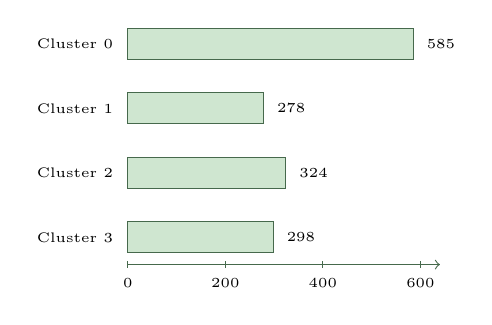
\begin{tikzpicture}[x=0.0062cm,y=0.82cm,font=\tiny]
                \foreach \cluster/\records/\position in
                    {0/585/3,1/278/2,2/324/1,3/298/0} {
                    \fill[chartgreen]
                        (0,\position) rectangle (\records,\position+0.48);
                    \draw[chartgreenline]
                        (0,\position) rectangle (\records,\position+0.48);
                    \node[anchor=east] at (-10,\position+0.24)
                        {Cluster \cluster};
                    \node[anchor=west] at (\records+8,\position+0.24)
                        {\records};
                }
                \draw[->,chartgreenline] (0,-0.18) -- (640,-0.18);
                \foreach \tick in {0,200,400,600} {
                    \draw[chartgreenline]
                        (\tick,-0.23) -- (\tick,-0.13);
                    \node[anchor=north] at (\tick,-0.25) {\tick};
                }
            \end{tikzpicture}
        \end{column}
    \end{columns}

    \vspace{0.35cm}
    \begin{minipage}{0.94\textwidth}
        \scriptsize
        Cluster 0 contained the largest share of records. The other three
        clusters each contained approximately 19--22\% of the held-out
        dataset. Cluster labels are optimizer identifiers, not clinical
        patient categories.
    \end{minipage}
\end{frame}

\begin{frame}[t]{PRTI-GH: Minimum Entropy Values Across Clusters}
    \scriptsize
    \centering
    \textbf{All 77 sensitive attributes were evaluated in every cluster}

    \vspace{0.22cm}
    \begin{columns}[T,onlytextwidth]
        \begin{column}{0.58\textwidth}
            \centering
            \renewcommand{\arraystretch}{1.18}
            \setlength{\tabcolsep}{3.5pt}
            \begin{tabular}{crr}
                \toprule
                \textbf{Cluster} &
                \begin{tabular}[c]{@{}c@{}}\textbf{Attributes whose lowest}\\[-1pt]
                    \textbf{entropy occurred here}\end{tabular} &
                \begin{tabular}[c]{@{}c@{}}\textbf{Sum of selected}\\[-1pt]
                    \textbf{minimum entropies}\end{tabular} \\
                \midrule
                0 & 15 & 9.507942 \\
                1 & 27 & 34.954852 \\
                2 & 13 & 17.197126 \\
                3 & 22 & 38.065515 \\
                \midrule
                \textbf{Total} & \textbf{77} & \textbf{99.725436} \\
                \bottomrule
            \end{tabular}
        \end{column}

        \begin{column}{0.40\textwidth}
            \centering
            \textbf{Attributes supplying the minimum}

            \vspace{0.15cm}
            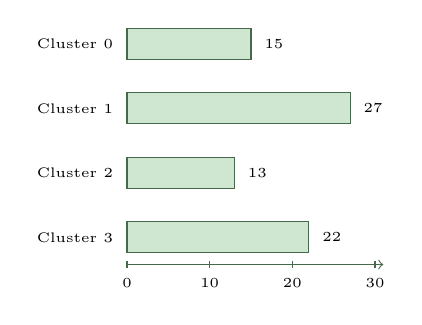
\begin{tikzpicture}[x=0.105cm,y=0.82cm,font=\tiny]
                \foreach \cluster/\attributes/\position in
                    {0/15/3,1/27/2,2/13/1,3/22/0} {
                    \fill[chartgreen]
                        (0,\position) rectangle (\attributes,\position+0.48);
                    \draw[chartgreenline]
                        (0,\position) rectangle (\attributes,\position+0.48);
                    \node[anchor=east] at (-0.5,\position+0.24)
                        {Cluster \cluster};
                    \node[anchor=west] at (\attributes+0.45,\position+0.24)
                        {\attributes};
                }
                \draw[->,chartgreenline] (0,-0.18) -- (31,-0.18);
                \foreach \tick in {0,10,20,30} {
                    \draw[chartgreenline]
                        (\tick,-0.23) -- (\tick,-0.13);
                    \node[anchor=north] at (\tick,-0.25) {\tick};
                }
            \end{tikzpicture}
        \end{column}
    \end{columns}

    \vspace{0.28cm}
    \begin{minipage}{0.96\textwidth}
        \scriptsize
        For each sensitive attribute, the method selected the smallest of
        its four cluster entropy values. Fifteen of the 77 selected minima
        came from Cluster 0, 27 from Cluster 1, 13 from Cluster 2, and 22
        from Cluster 3. Their sum is $99.7254355715$. No sensitive attribute
        was removed from any cluster.
    \end{minipage}
\end{frame}

\begin{frame}[t]{PRTI-GH: Re-identification Risk Evaluation}
    \scriptsize
    \centering
    \textbf{(d) Measured sample-based risk before and after anonymization}

    \vspace{0.3cm}
    \renewcommand{\arraystretch}{1.22}
    \setlength{\tabcolsep}{5pt}

    \begin{tabular*}{0.84\textwidth}{@{}@{\extracolsep{\fill}}lrr@{}}
        \toprule
        \textbf{Risk metric} & \textbf{Before} & \textbf{After} \\
        \midrule
        Equivalence classes
            & 1,481 & 4 \\
        Maximum prosecutor risk
            & 100.0000\% & 0.3597\% \\
        Median prosecutor risk
            & 100.0000\% & 0.3086\% \\
        Marketer risk
            & 99.7306\% & 0.2694\% \\
        Expected correct marketer matches
            & 1,481 & 4 \\
        Records with risk above 5\%
            & 1,485 & 0 \\
        Records with risk above 7.5\%
            & 1,485 & 0 \\
        Records with risk above 10\%
            & 1,485 & 0 \\
        \bottomrule
    \end{tabular*}

    \vspace{0.35cm}
    \begin{minipage}{0.94\textwidth}
        \scriptsize
        \textit{Interpretation:} Prosecutor risk for a record is the reciprocal
        of its equivalence-class size. Marketer risk is $G/N$, where $G$ is
        the number of equivalence classes and $N=1{,}485$. Mean prosecutor
        risk is omitted because it equals the sample-based marketer risk.

        \vspace{0.2cm}
        \textit{Limitation:} Journalist risk is not estimated because the
        population QID frequencies and sampling fraction are unavailable.
    \end{minipage}
\end{frame}

\begin{frame}[t]{PRTI-GH: Selected Held-out Result}
    \scriptsize
    \centering

    \textbf{Predeclared selected configuration evaluated on held-out seed 12}

    \vspace{0.35cm}
    \renewcommand{\arraystretch}{1.25}
    \setlength{\tabcolsep}{3pt}

    \begin{tabular*}{\textwidth}{@{}@{\extracolsep{\fill}}clccccc@{}}
        \toprule
        \textbf{\# of clusters} & \textbf{Hyperparameter values} & \textbf{IL} &
        \textbf{$\tau=0.05$} & \textbf{$\tau=0.075$} &
        \textbf{$\tau=0.10$} & \textbf{HA} \\
        \midrule
        \rowcolor{lightblue}
        4 & $(k=16,\ \lambda=0.0000002,\ n_c=4)$ &
        \textbf{0.4602} & \textbf{0} & \textbf{0} & \textbf{0} & \textbf{0} \\
        \bottomrule
    \end{tabular*}

    \vspace{0.45cm}
    \begin{block}{Held-out evidence}
        \begin{itemize}
            \item Full information loss: $0.460240739862$.
            \item Entropy sum: $99.7254355715$; objective value: $0.460220794775$.
            \item Four equivalence classes with sizes 585, 278, 324, and 298.
            \item Minimum achieved class size: 278, exceeding the configured $k=16$.
            \item Zero linkage exposure at all three thresholds and zero
            homogeneity-exposed records.
        \end{itemize}
    \end{block}

    \vspace{0.2cm}
    \begin{minipage}{0.96\textwidth}
        \scriptsize
        The held-out result is reported separately because seed 12 was not
        used to choose the configuration. Tables (a) and (b) are descriptive
        summaries of comparison seeds 0, 1, and 2.
    \end{minipage}
\end{frame}

\begin{frame}[t]{PRTI-GH: Overall Distribution Evaluation}
    \scriptsize
    \centering
    \textbf{(e) Dataset-wide distribution similarity before and after anonymization}

    \vspace{0.22cm}
    \renewcommand{\arraystretch}{1.18}
    \setlength{\tabcolsep}{4pt}

    \begin{tabular*}{\textwidth}{@{}@{\extracolsep{\fill}}lrrrrrr@{}}
        \toprule
        \textbf{Scope} & \textbf{Attributes} & \textbf{Numeric} &
        \textbf{Categorical} & \textbf{Missing before} &
        \textbf{Missing after} & \textbf{Similarity} \\
        \midrule
        Overall dataset      & 106 & 17 & 89 & 4.65\% & 4.78\% & 0.8857 \\
        Quasi-identifiers    &  29 &  2 & 27 & 2.32\% & 2.80\% & 0.5822 \\
        Sensitive attributes & 77 & 15 & 62 & 5.53\% & 5.53\% & 1.0000 \\
        \bottomrule
    \end{tabular*}

    \vspace{0.35cm}
    \begin{tabular*}{\textwidth}{@{}@{\extracolsep{\fill}}lrrrrrrrr@{}}
        \toprule
        & \multicolumn{2}{c}{\textbf{Wasserstein}} &
        \multicolumn{2}{c}{\textbf{KS}} &
        \multicolumn{2}{c}{\textbf{Total variation}} &
        \multicolumn{2}{c}{\textbf{Jensen--Shannon}} \\
        \cmidrule(lr){2-3}\cmidrule(lr){4-5}\cmidrule(lr){6-7}\cmidrule(lr){8-9}
        \textbf{Scope} & \textbf{Mean} & \textbf{Max.} &
        \textbf{Mean} & \textbf{Max.} & \textbf{Mean} & \textbf{Max.} &
        \textbf{Mean} & \textbf{Max.} \\
        \midrule
        Overall dataset       & 0.0185 & 0.2499 & 0.0465 & 0.5690 & 0.1209 & 0.9663 & 0.1389 & 0.9546 \\
        Quasi-identifiers     & 0.1574 & 0.2499 & 0.3956 & 0.5690 & 0.3985 & 0.9663 & 0.4580 & 0.9546 \\
        Sensitive attributes & 0.0000 & 0.0000 & 0.0000 & 0.0000 & 0.0000 & 0.0000 & 0.0000 & 0.0000 \\
        \bottomrule
    \end{tabular*}

    \vspace{0.28cm}
    \begin{minipage}{0.97\textwidth}
        \tiny
        \textit{Notes:} Numeric attributes use normalized Wasserstein and KS
        distances; categorical attributes use total variation and
        Jensen--Shannon distances. Similarity is one minus the equally weighted
        mean attribute distance. The overall score is reported with the QID
        score because the 77 unchanged sensitive attributes raise the overall
        similarity. Missingness increased only for the QID
        \texttt{presenceOfSupervisionsRoadGuideF}, from 1,001 to 1,207 missing
        values; sensitive-attribute missingness was unchanged.
    \end{minipage}
\end{frame}

\end{document}
